\section{Módulo Especializado: Objetos Perdidos y Solidaridad Estudiantil}
\label{sec:objetos_perdidos}

En comunidades universitarias masivas, los canales de mensajería instantánea trascienden la consulta académica formal y operan frecuentemente como redes solidarias de auxilio cotidiano. Entre las dinámicas emergentes más representativas destaca el reporte y recuperación de objetos extraviados en las instalaciones de la Carrera de Informática. La integración de esta funcionalidad dentro de SentiDataUMSA resuelve un desafío doble: metodológicamente, exige discriminar mediante técnicas de procesamiento del lenguaje natural (PLN) las menciones literales de pérdidas físicas frente a usos metafóricos recurrentes; tecnológicamente, proporciona a los estudiantes y administradores un tablón reactivo para la búsqueda y restitución de bienes.

\subsection{Detección Semántica y Depuración de Ambigüedades}

La identificación automática de incidentes de extravío requirió el diseño de un filtro de desambiguación semántica basado en patrones sintácticos dirigidos. Expresiones coloquiales como ``\emph{ya perdí la materia}'', ``\emph{no quiero perder el semestre}'' o ``\emph{encontré un error en el código}'' comparten lemas con los eventos de interés (\textit{perder}, \textit{encontrar}), pero carecen de correlato material.

Para garantizar una precisión estricta, se formuló una regla de filtrado en dos etapas:
\begin{enumerate}[label=\arabic*)]
  \item \textbf{Filtrado Léxico Positivo:} Detección de combinaciones entre verbos de pérdida o hallazgo y sustantivos pertenecientes al inventario léxico de bienes personales portables (\textit{cargador}, \textit{mochila}, \textit{carnet}, \textit{celular}, \textit{cuaderno}, \textit{chompa}, \textit{calculadora}, \textit{audífonos}, \textit{llaves}).
  \item \textbf{Exclusión Contextual:} Descarte automatizado de enunciados con colocaciones curriculares (\textit{materia}, \textit{semestre}, \textit{auxiliatura}, \textit{cupo}, \textit{parcial}).
\end{enumerate}

Este procedimiento aisló un subcorpus verificado de 53 eventos físicos sobre los 23.371 mensajes del histórico. Del total, 38 correspondieron a declaraciones activas de pérdida (71,7\%) y 15 a reportes de hallazgo solidario por parte de compañeros o personal de planta (28,3\%).

\begin{table}[htbp]
  \centering
  \small
  \caption{Distribución por Categoría de Objeto y Ubicación Espacial en el Módulo de Objetos Perdidos}
  \label{tab:objetos_perdidos}
  \resizebox{\textwidth}{!}{
  \begin{tabular}{llrrlrr}
    \toprule
    \multicolumn{3}{c}{\textbf{Tipología de Objeto}} & \multicolumn{3}{c}{\textbf{Ubicación Espacial en el Edificio}} \\
    \cmidrule(lr){1-3} \cmidrule(lr){4-6}
    Categoría & Ejemplos & Casos (\%) & Espacio Físico & Detalle & Casos (\%) \\
    \midrule
    Cargadores / Cables    & USB-C, adaptadores lap. & 16 (30,2\%) & Piso 4       & Labs Computación / Redes & 18 (34,0\%) \\
    Cuadernos / Útiles     & Cuaderno apuntes, calc. & 14 (26,4\%) & Piso 3       & Lab LASIN / Aulas 301--305 & 14 (26,4\%) \\
    Documentos / Carnets   & C.I., matrícula UMSA    & 12 (22,6\%) & Piso 2 / PB  & Auditorio / Biblioteca   & 11 (20,8\%) \\
    Móviles / Accesorios   & Smartphones, estuches  & 7 (13,2\%)  & Áreas Comunes& Gradas, pasillos, quiosco & 6 (11,3\%) \\
    Prendas de Vestir      & Chompas, bufandas       & 4 (7,5\%)   & No Declarado & Sin referencia espacial  & 4 (7,5\%)  \\
    \midrule
    \textbf{Total Corpus}  & \textit{Objetos físicos}& \textbf{53 (100\%)} & \textbf{Total} & \textit{Monitoreo campus} & \textbf{53 (100\%)} \\
    \bottomrule
  \end{tabular}
  }
  \vspace{4pt}
  \begin{minipage}{0.95\textwidth}
    \footnotesize
    \textit{Nota.} Datos depurados tras eliminar falsos positivos de expresiones ambiguas (e.g., ``\emph{perder la materia}'', ``\emph{encontrar el aula}''). Se identificaron 38 declaraciones de pérdida (71,7\%) y 15 notificaciones de hallazgo solidario (28,3\%).
  \end{minipage}
\end{table}


\subsection{Distribución Espacial, Tipología y Estacionalidad}

El análisis descriptivo de las menciones reveló patrones espaciales y temporales altamente consistentes con la infraestructura física y el calendario institucional de la Carrera de Informática (Tabla~\ref{tab:objetos_perdidos}):
\begin{itemize}
  \item \textbf{Zonas Críticas (Hotspots):} El Piso 4 concentra el 34,0\% de los extravíos (18 casos), atribuible a la alta rotación de estudiantes en los laboratorios de cómputo y redes. El Piso 3, sede del Laboratorio de Sistemas e Informática (LASIN) y de las aulas 301 a 305, registra el 26,4\% de los incidentes (14 casos). Los pisos inferiores (Piso 2, Planta Baja, Biblioteca y Auditorio) acumulan en conjunto el 20,8\% (11 casos).
  \item \textbf{Tipología de Bienes:} Los accesorios tecnológicos (cargadores USB-C, adaptadores de portátiles y cables) encabezan la nómina con el 30,2\% (16 casos), seguidos de cuadernos de apuntes y calculadoras científicas (26,4\%, 14 casos) y documentos institucionales críticos como cédulas de identidad o matrículas universitarias (22,6\%, 12 casos).
  \item \textbf{Concentración Estacional:} Tal como se evidencia en la telemetría temporal, el 47,1\% de los extravíos se produce de forma concentrada durante los cursos intensivos de temporada (Invierno y Verano) y las semanas de evaluaciones finales, períodos caracterizados por jornadas extensas de permanencia y elevados niveles de fatiga cognitiva.
\end{itemize}

\begin{figure}[htbp]
  \centering
  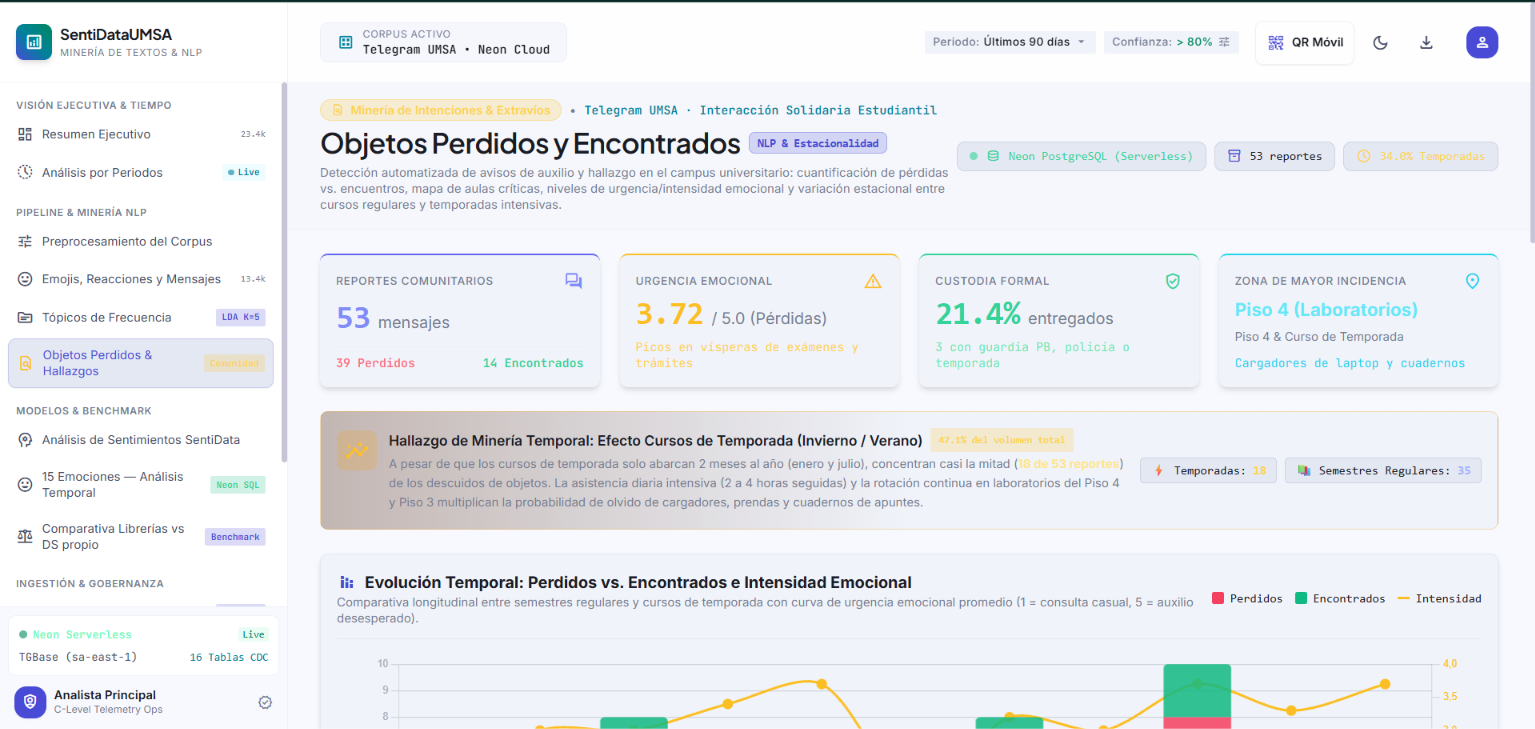
\includegraphics[width=0.92\textwidth]{figures/CAP15JNAC.png}
  \vspace{4pt}
  \caption{Panel analítico general del módulo de Objetos Perdidos y Encontrados en SentiDataUMSA.}
  \label{fig:ui_obj_overview}
\end{figure}

\begin{figure}[htbp]
  \centering
  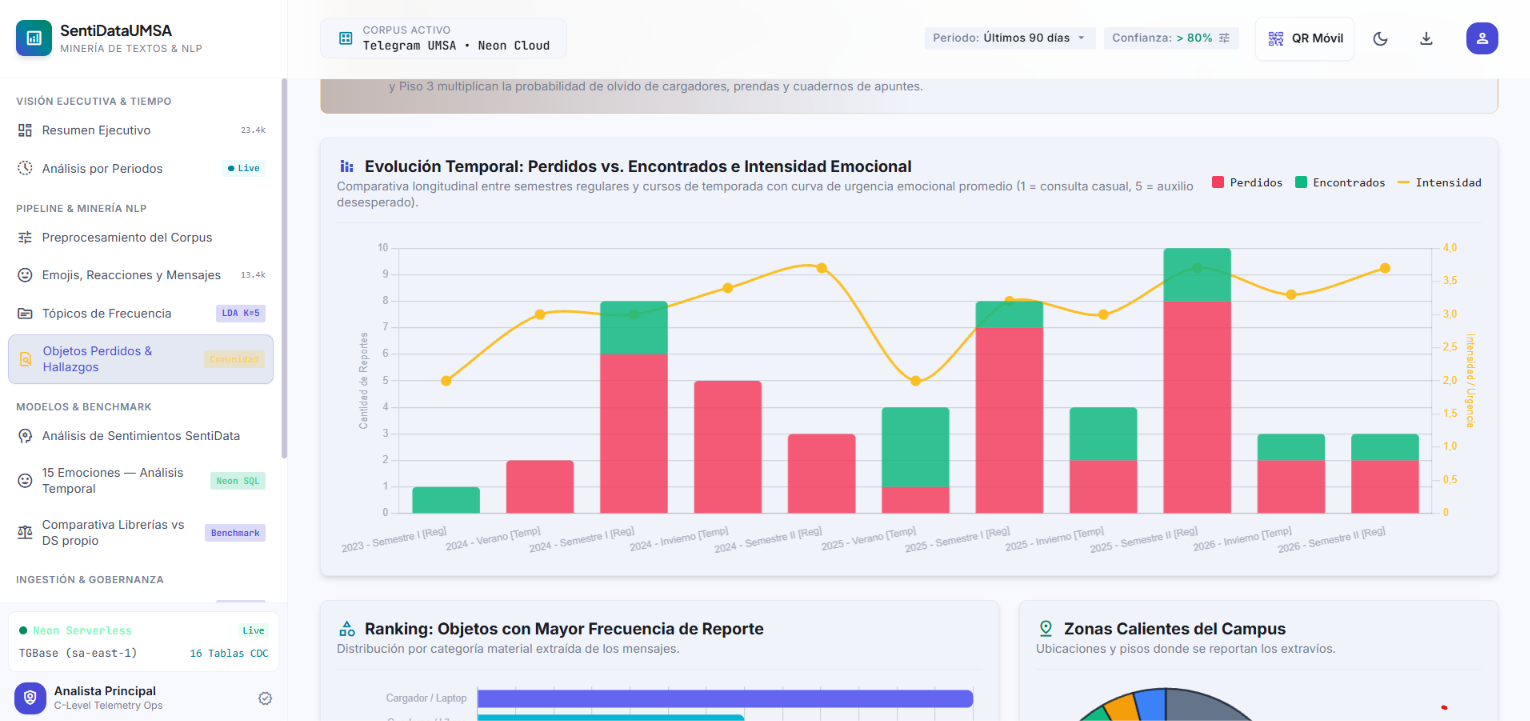
\includegraphics[width=0.92\textwidth]{figures/CAP16JNAC.png}
  \vspace{4pt}
  \caption{Concentración estacional de extravíos con un pico del 47,1\% en períodos de exámenes y cursos de temporada.}
  \label{fig:ui_obj_temporal}
\end{figure}

\begin{figure}[htbp]
  \centering
  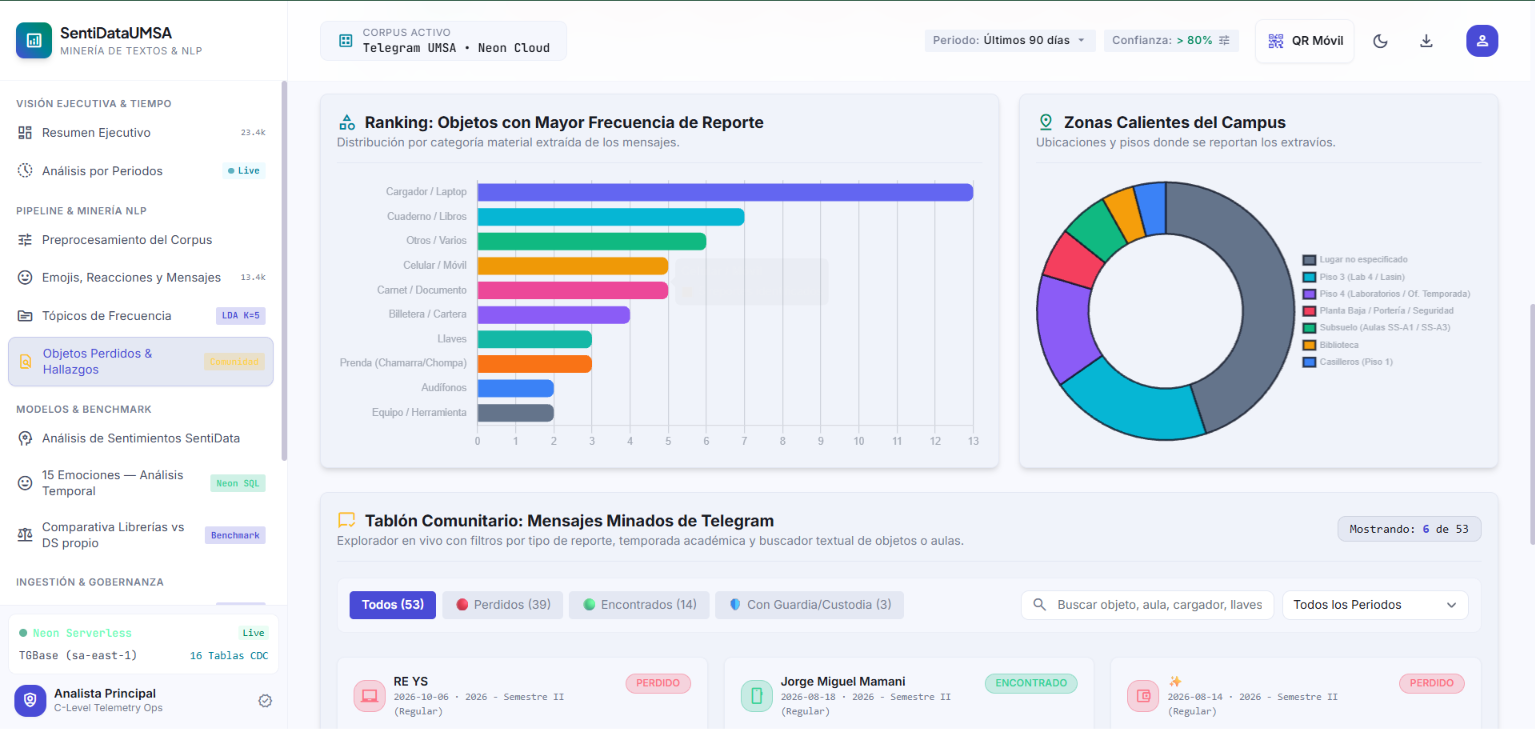
\includegraphics[width=0.92\textwidth]{figures/CAP17JNAC.png}
  \vspace{4pt}
  \caption{Distribución espacial de pérdidas por pisos del edificio y clasificación por tipología de objeto.}
  \label{fig:ui_obj_ranking}
\end{figure}

\subsection{Implementación de la Interfaz Reactiva y Paginación Progresiva}

Para garantizar una experiencia de usuario fluida y evitar la saturación visual ante listados extensos, la interfaz de consulta implementa un tablón interactivo de avisos con renderizado asíncrono y paginación progresiva en bloques de seis elementos (Figura~\ref{fig:ui_obj_tablon}). 

\begin{figure}[htbp]
  \centering
  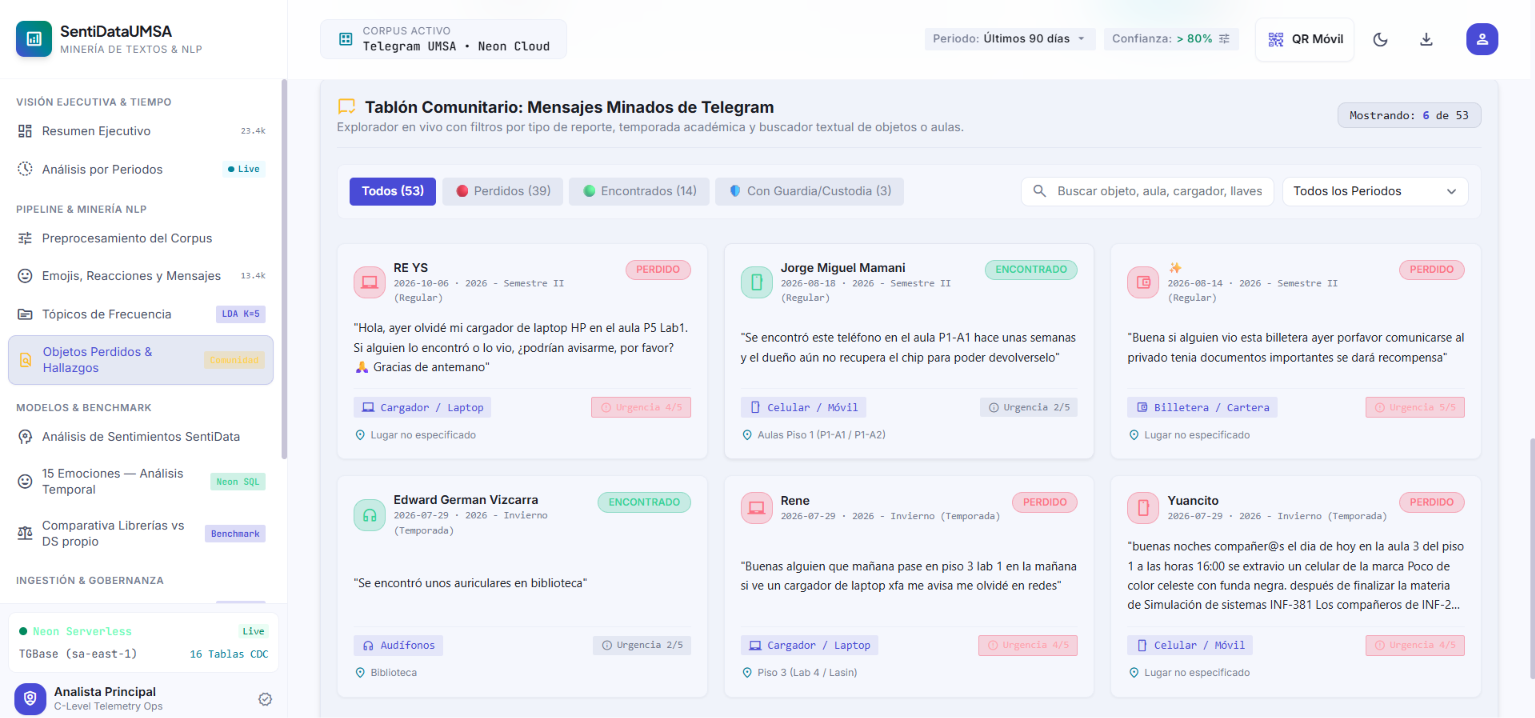
\includegraphics[width=0.92\textwidth]{figures/CAP18JNAC.png}
  \vspace{4pt}
  \caption{Tablón interactivo de avisos de objetos perdidos con paginación progresiva de 6 en 6 y filtros reactivos.}
  \label{fig:ui_obj_tablon}
\end{figure}

El componente cliente (\texttt{objetos\_perdidos.html}) consume un endpoint especializado (\texttt{/api/v1/objetos-perdidos}) que soporta filtrado reactivo por tipo de reporte (todos, perdidos, encontrados), búsqueda en texto completo por palabras clave de objeto o ubicación, y ordenamiento cronológico. Al cargar la vista, el sistema presenta los seis registros más recientes con distintivos visuales de estado y etiquetas de piso, ofreciendo el botón dinámico \emph{Mostrar más} para cargar incrementalmente los registros restantes sin recargar la página.
